%%%%%%%%%%%%%%%%%%%%%%%%%%%%%%%%%%%%%%%%%%%%%%%%%%%%%%%%%%%%%%%%%%%%%%%%%%%
%
% Template for a LaTex article in Slovak.
%
%%%%%%%%%%%%%%%%%%%%%%%%%%%%%%%%%%%%%%%%%%%%%%%%%%%%%%%%%%%%%%%%%%%%%%%%%%%

\documentclass{article}

\usepackage[utf8]{inputenc}
\usepackage[slovak]{babel}
\usepackage[document]{ragged2e}
\usepackage{amsmath}
\usepackage{siunitx}
\usepackage{multicol}
\usepackage{textcomp}
\usepackage{amsmath, amsthm, amsfonts}
\usepackage{graphicx}
\usepackage{url}
\usepackage{subcaption}

% Theorems
%-----------------------------------------------------------------
\newtheorem{thm}{Theorem}[section]
\newtheorem{cor}[thm]{Corollary}
\newtheorem{lem}[thm]{Lemma}
\newtheorem{prop}[thm]{Proposition}
\theoremstyle{definition}
\newtheorem{defn}[thm]{Definition}
\theoremstyle{remark}
\newtheorem{rem}[thm]{Remark}

% Shortcuts.
% One can define new commands to shorten frequently used
% constructions. As an example, this defines the R and Z used
% for the real and integer numbers.
%-----------------------------------------------------------------
\def\RR{\mathbb{R}}
\def\ZZ{\mathbb{Z}}

% Similarly, one can define commands that take arguments. In this
% example we define a command for the absolute value.
% -----------------------------------------------------------------
\newcommand{\abs}[1]{\left\vert#1\right\vert}

% Operators
% New operators must defined as such to have them typeset
% correctly. As an example we define the Jacobian:
% -----------------------------------------------------------------
\DeclareMathOperator{\Jac}{Jac}

%-----------------------------------------------------------------
\title{Newtonová metóda riešenie rovníc}
\author{Miroslav Kurka\\
  \small Dept. of Biophysics\\
  \small Pavol Jozef Šafárik University in Košice\\
  \small Slovakia 
}

\begin{document}
\maketitle


\section{Úloha}
Nájdite riešenie diferenciálnej rovnice (počiatočnej úlohy)

$$\frac{dy}{dx}= \frac{x}{y^3}$$

kde $y(1) = 1$ je hodnota $y$ v bode $x = 1$.
Rovnicu riešte:
\begin{itemize}
  \item Eulerovou metódou
  \item Heunovou metódou
\end{itemize}

s krokom $dx = 0.1$ a $dx = 0.01$ pre interval $[a, b] = [1, 10]$ a výsledné riešenia
porovnajte s výsledkom obdŕžaným pomocou zabudovanej funkcie $lsode$ v prostredí
Octave.
Nakoniec numerické výsledky porovnajte s presným riešením
$y = (2x^2-1)^{1/4}$
a výsledky zobrazte do spoločných grafov v tvare rozdielu medzi presným riešením
a približnými (numerickými) riešeniami


\subsection{Teória}\label{sec:nothing}
Úloha je založená na riešení diferenciálnej rovnice pomocou Runge-Kutta (RK) metód. Tie používajú aproximaciu derivacií kombináciou hodnôt funkcie $f$ v niekoľkých strategických bodoch na intervale $[t_n, t_{n+1}]$\cite{Zukovic}. Všeobecne sú dané rekurentným vzťahom:
$$y_{n+1}=y_n+h_n\sum_{i=1}^r \alpha_i k_i$$
\subsubsection{Eulerova metóda}
Jedná sa o RK metódu prvého rádu. Metóda je založená na princípe nahradenia krivky $y=f(x)$ jej dotyčnicou v bode $[x_i,f(x_i)]$ na intervale $⟨x_i,x_i+1⟩$. Keďže smernicu dotyčnice vieme vypočítať pomocou derivácie funkcie t.j. $k=y'(x_i)=f(x_i,y_i)$, dostávame rekurentný vzorec pre výpočet hodnoty funkcie v bode $y_{i+1}$\cite{Web}:
$$y_{i+1}=y_i+hf(x_i,y_i)$$
kde $h = x_{i+1}-x_i$ je krok metódy.

\subsubsection{Heuneho metóda}
Je to RK metóda druhého rádu. Rozdiel s Eulerovou metódou je, že pri odvodení sa funkcia v integrály nahrádza Lagrangeovým interpolačným polynómom prvého stupňa\cite{Web}. Následne platí rekurentný vzorec: 
$$y_{n+1} = y_n + h_n/2 (k_1+k_2)$$
 , kde $k_2 =f(x_n+1,y_n+h_n k_1)$ a $k_1 =f(x_n,y_n)$.
\subsection{Algoritmus}
V našej implementácií najprv inicializujeme funkciu ktorú chceme aproximovať a počet bodov N=10 zo zadania\footnote{Zo zadania mi nebolo celkom jasné či ide o [1,10] v zmysle matlab poľa tj. 10 bodov alebo interval v matematike viz. matlab zdrojak.} . Následne zavedieme krok intervalu v našom prípade dx\footnote{značenie ponechávame podľa cvičení} v teórii vyššie je to $h$. Potom nastavíme polia na ukladanie hodnôt pre body $x$ a pre výsledky v bodoch $x$ pre rekurentné vzťahy Eulerovej, Heuneho metóde a pre analytické riešenie diferenciálnej rovnice. Podľa zadania nastavíme prvý bod 1 a funkčnú hodnotu pre všetky prípady tiež ako 1. Vo for slučke v každom kroku aktualizujeme hodnotu bodu $x(i+1)$ o krok $dx$ tj. Vypočítame nasledujúci bod. Ďalej sa podľa vzorca Eulerovej metódy z teórie vypočíta hodnota riešenia $y\_(euler)(i+1)$. K výpočtu Heuneho metódy potrebujeme hodnoty $k_1$ a $k_2$. Pre prehľadnosť riešenia sa inicializuje $y\_temp$ = $k_2$ . Tato predpočítaná hodnota je následne dosadená do rekurentného vzťahu Heuneho metódy pre bod $x\_i$. Ako posledný krok sa vypočíta hodnota exaktného riešenia dif. rovnice pre následne porovnanie. Všetky hodnoty sa ukladajú do poli, ktoré sme si pripravili. 
\subsection{Výsledky}
Na Obr.\ref{fig:dx01} sú zobrazene riešenia pre väčší krok intervalu. Z grafu vidíme, že Eulerova metóda pri intervale 10 bodov kde podintervaly sú väčšie ma vyššiu chybu aproximácie ako Heuneho metóda.
\begin{figure}
  \centering
  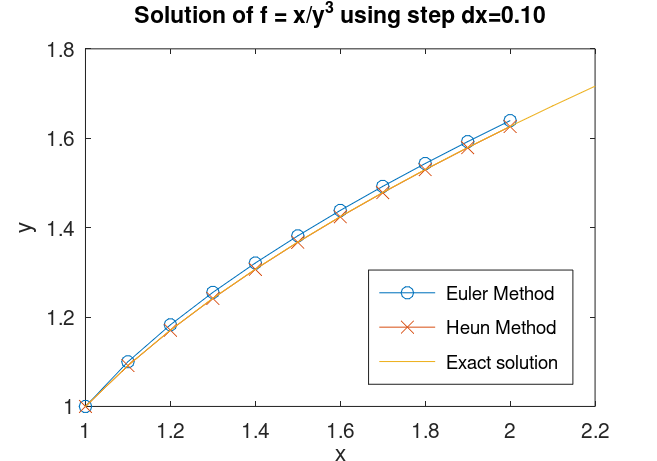
\includegraphics[width=1\textwidth]{dx01.png}
  \caption{Graf riešenií metód s krokom dx=0.1}
  \label{fig:dx01}
\end{figure}

Z Obr.\ref{fig:dx001} je zrejmé, že pri zväčšení kroku intervalu sa aproximácia pomocou Eulerovej metódy zlepšila a to z dôvodu, že veľkosti podintervalov v intervale 10 bodov sa výrazne zmenšili. Avšak opäť Heuneho metóda poskytuje presnejšie riešenie. Tento výsledok je zrejmý z teórie.
\begin{figure}
  \centering
  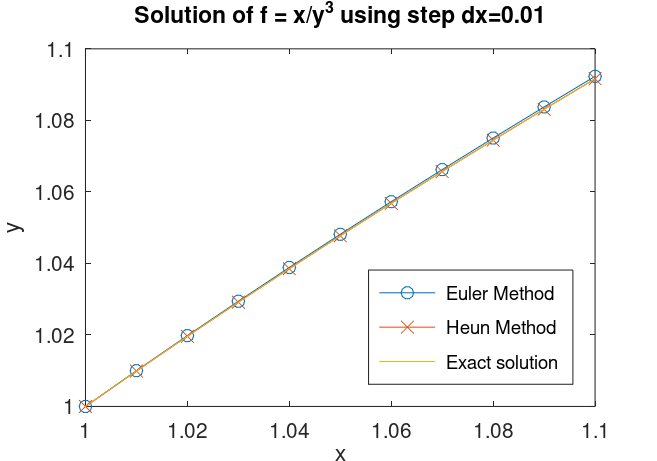
\includegraphics[width=1\textwidth]{dx001.png}
  \caption{Graf riešenií metód s krokom dx=0.01}
  \label{fig:dx001}
\end{figure}


\begin{figure}[h]
  \centering
  \begin{subfigure}[b]{0.49\textwidth}
    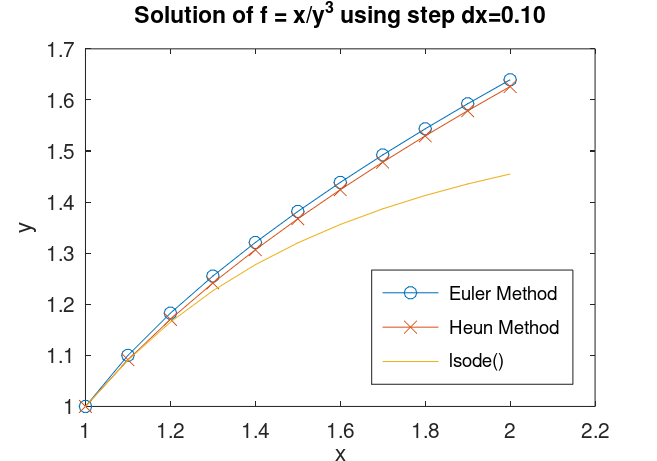
\includegraphics[width=\textwidth]{lsode01.png}
    \caption{Vysoká odchylka pri kroku intervalu 0.1}
  \end{subfigure}
  \hfill
  \begin{subfigure}[b]{0.49\textwidth}
    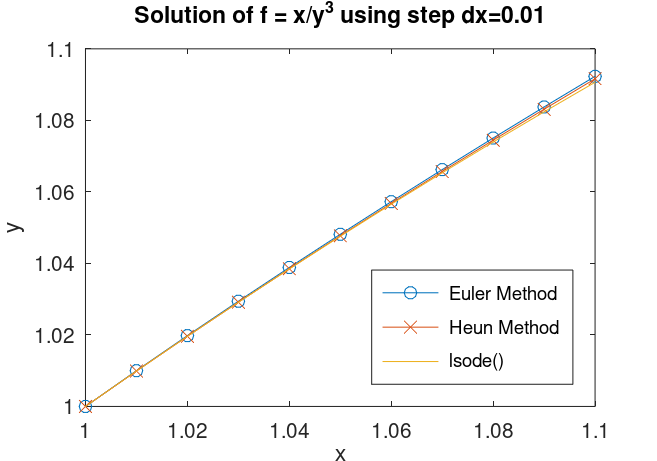
\includegraphics[width=\textwidth]{lsode.png}
    \caption{Nízka odchylka pri kroku intervalu 0.01}
  \end{subfigure}
  \caption{Porovnanie lsode() a analytického riešenia s rozlyčnými krokmi intervalu}
\end{figure}

\begin{figure}[h]
  \centering
  \begin{subfigure}[b]{0.49\textwidth}
    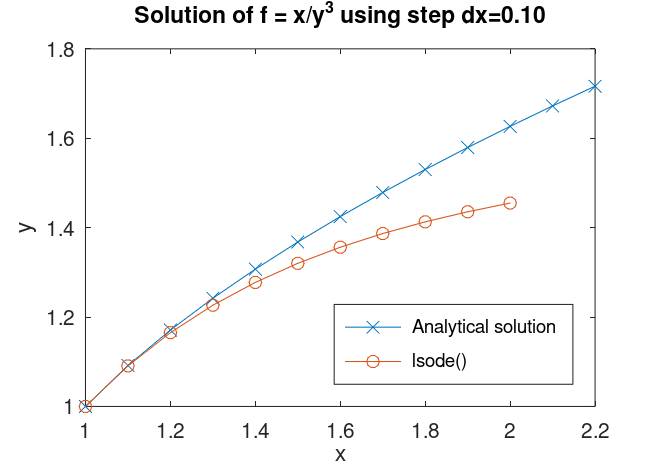
\includegraphics[width=\textwidth]{analytical.png}
    \caption{Krok intervalu 0.1 vykazuje vyššiu chybu}
  \end{subfigure}
  \hfill
  \begin{subfigure}[b]{0.49\textwidth}
    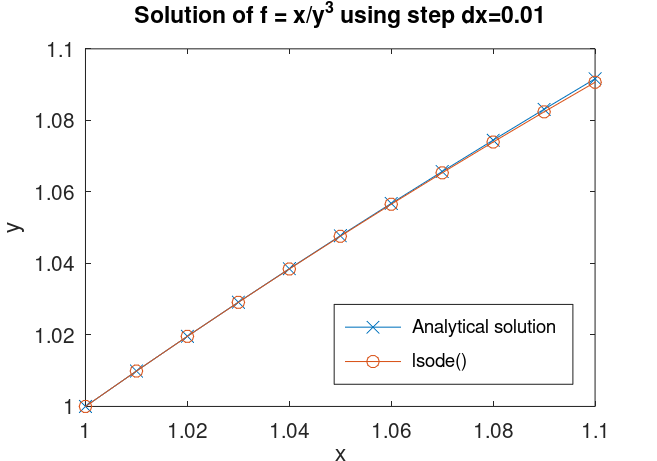
\includegraphics[width=\textwidth]{analytical_pre.png}
    \caption{Krok intervalu 0.01 vykazuje lepšiu aproximáciu}
  \end{subfigure}
  \caption{Porovnanie lsode() a analytického riešenia s rozlyčnými krokmi intervalu}
  \label{fig:analyticallsode}
\end{figure}
Pri riešení diferenciálnej rovnice pomocou vstavenej metódy $lsode()$ je pri kroku $dx=0.01$ riešenie takmer totožné s Heuneho a Eulerovou metódou. Pri zväčšení kroku avšak nastáva vysoká chyba medzi riešeniami. V grafe na Obr. \ref{fig:analyticallsode} vidíme porovnanie analytického riešenia a $lsode()$ pri kroku $dx=0.1$, ktoré sa tiež výrazne líšia. Dôvodom môže byt zle použitie funkcie lsode() v kóde alebo chyba nasej implementácie. 

\pagebreak






% Bibliography
%-----------------------------------------------------------------
\begin{thebibliography}{99}
\bibitem{Web} \emph{Eulerova a Heunova metóda} Dostupné z \url{http://matematikabezproblemov.webjet.sk/domov/studijne-materialy/matematika-vs/numericka-matematika/eulerova-heunova-metoda/}
\bibitem{Zukovic}Žukovič, M. (2015) \emph{Počítačová fyzika I} Dostupné z \url{https://ufv.science.upjs.sk/zukovic/download/POF1/Literatura/Pocitacova%20fyzika%20I.pdf}
\end{thebibliography}

\end{document}
